\documentclass[10pt]{beamer}

\usetheme[progressbar=frametitle, numbering=fraction,]{metropolis}

\usepackage{booktabs}
\usepackage[scale=2]{ccicons}

\usepackage{pgfplots}
\usepgfplotslibrary{dateplot}

\usepackage{xspace}
\newcommand{\themename}{\textbf{\textsc{metropolis}}\xspace}

\title{Near-optimal probabilistic
RNA-seq quantification}
\subtitle{Bray and Pachter \emph{et al.} Nature biotechnology(2016)\\ doi:10.1038/nbt.3519}
\date{\today}
\author{Saket Choudhary}
\institute{}
\titlegraphic{}%\hfill
\includegraphics[height=1.5cm]{logo}}

\begin{document}

\maketitle
\begin{frame}[fragile]{RNA-Seq Workflow}
\begin{figure}
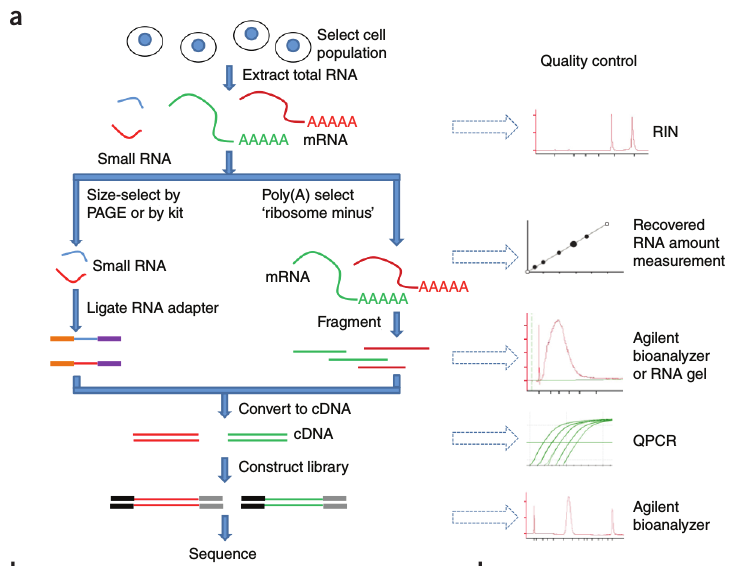
\includegraphics[width=\textwidth]{rnaseq-a}
\end{figure}
\footnotesize{Zheng and Mortazavi(2012)}
\end{frame}

\begin{frame}[fragile]{RNA-Seq Workflow}
\begin{figure}
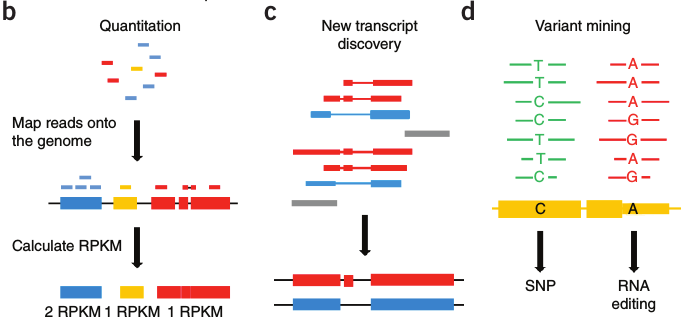
\includegraphics[width=\textwidth]{rnaseq-b}
\end{figure}
\footnotesize{Zheng and Mortazavi(2012)}
\end{frame}

\begin{frame}[fragile]{Motivation}

\begin{itemize}[<+-| alert@+>]
\item First two steps in typical RNA-Seq processing pipeline:
\begin{itemize}
\item Alignment
\item Quantification
\end{itemize}
\item Alignments are slow and probably not so important
\end{itemize}
\end{frame}

\begin{frame}[fragile]{It's all about compatible transcripts}

\begin{itemize}
\item Circumvent alignment step -- Use information from $k-mers$
\item Pseudoalignment: Find \emph{compatible} transcripts for a read, without pinpointing where exactly it aligns
%\item Overcoming difficulty of multi mapping reads -- 
\end{itemize}

\end{frame}

\begin{frame}[allowframebreaks]{Method}
\begin{figure}
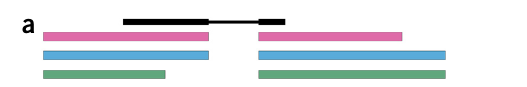
\includegraphics[width=\textwidth]{figa}
\caption{Reads and overlapping transcripts}
\end{figure}

\begin{figure}
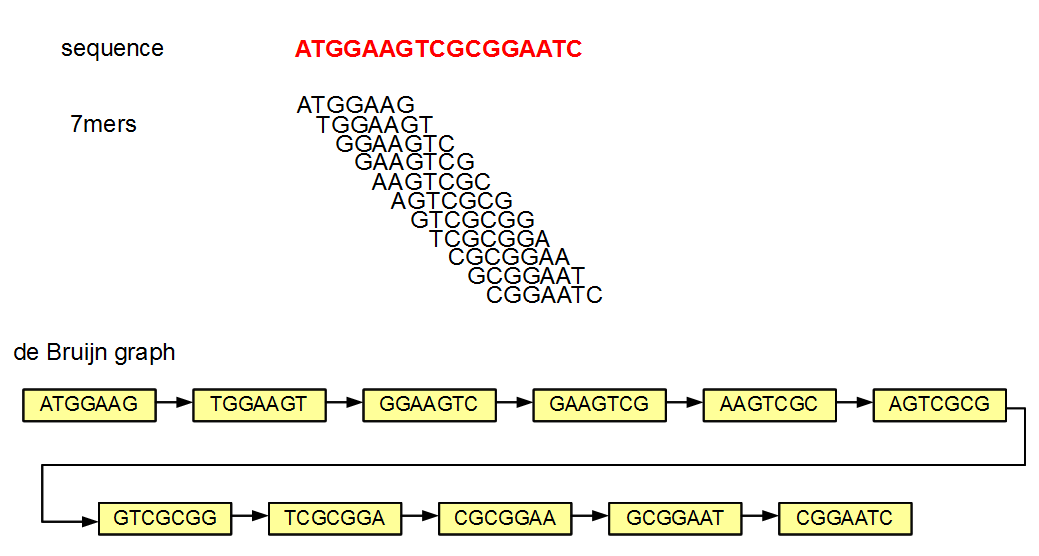
\includegraphics[width=\textwidth]{debruijn}
\caption{\footnotesize de Bruijn Graph}
\end{figure}

\begin{figure}
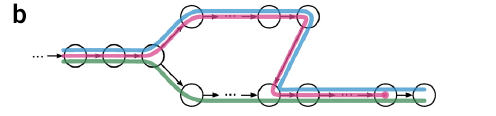
\includegraphics[width=\textwidth]{figb}
\caption{\footnotesize Transcriptome - de Bruijn Graph. Node = $k-mers$, Path = Transcript}
\end{figure}

\begin{figure}
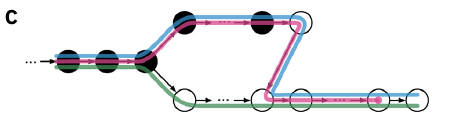
\includegraphics[width=\textwidth]{figc}
\caption{\footnotesize$k-mers$ in read = black nodes}
\end{figure}
\begin{figure}
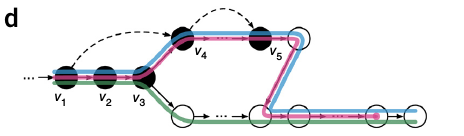
\includegraphics[width=\textwidth]{figd}
\caption{\footnotesize Nodes can be skipped if $k-mers$ did arise from blue transcript}
\end{figure}
\begin{figure}

\includegraphics[width=\textwidth]{fige}
\caption{\footnotesize Intersection of k-compatibility class}
\end{figure}
\begin{figure}
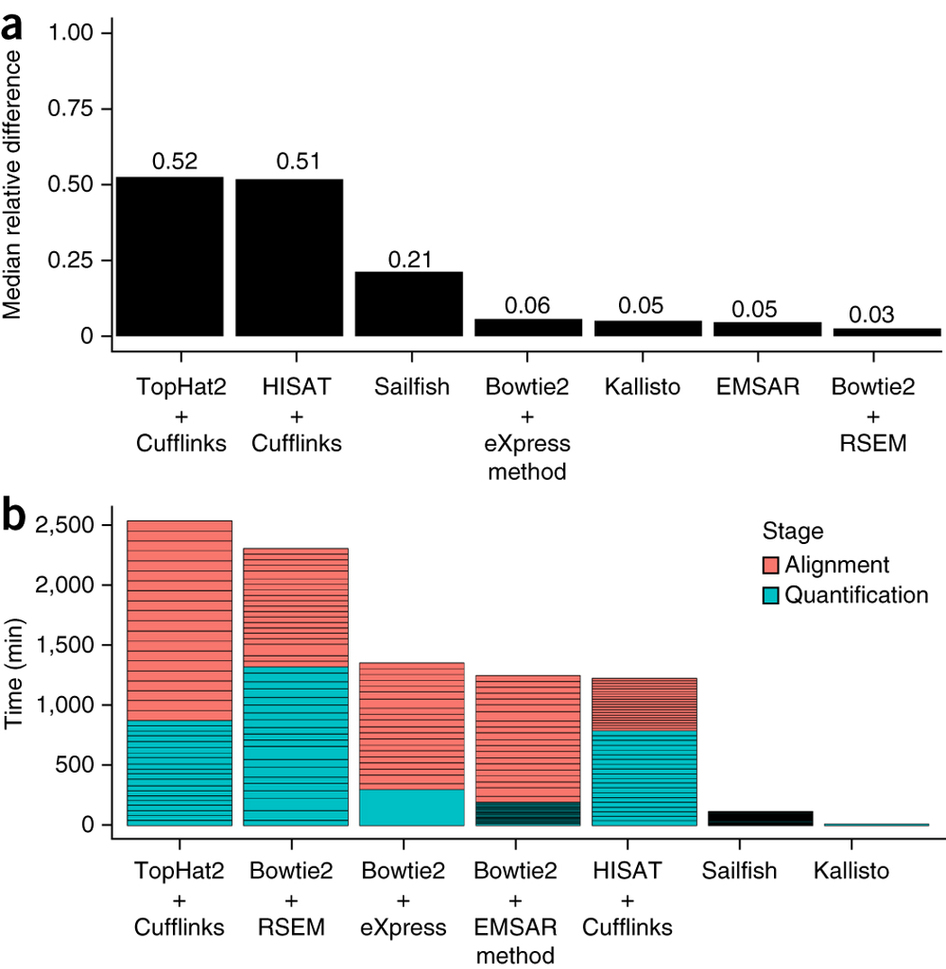
\includegraphics[scale=0.2]{comparison}
\caption{\footnotesize Quantification over a cup of coffee}
\end{figure}

\end{frame}


\begin{frame}[standout]
  Questions?
\end{frame}

\appendix


\begin{frame}{notes}
\begin{itemize}[<+-| alert@+>]
\item Better than \emph{Sailfish} that looks up $k-mers$ in reads into $k-mers$ of transriptome
\item Pseudoalignment: Find compatible transcript for a read, not where it exactly aligns
\item Key Idea: Find comtabile transcript for a read, not where it exactly aligns
\item Psuedoalignment: Subset  $S \subset T$ such that read $r$ is compatible.
\item Hash k-mers of reads and have a de-bruijn graph of transcriptome assembly handy
\item T-DBG: nodes are k-mers , each transcript corresponds to a path and path cover induces a k-comptability class for each k-mer
\item T-DBG: Colors correspond to transcripts, node corresponds to k-mers, every k-mer receives a color for each transcript it occurs in
\item Hash table stores mapping of each k-mer to the contig it is contained in
\end{itemize}

\end{frame}




%\begin{frame}[allowframebreaks]{References}

%  \bibliography{demo}
%  \bibliographystyle{abbrv}

%\end{frame}



\end{document}
